\documentclass{llncs}
\usepackage{graphicx}
\usepackage{url}
\usepackage{epsfig}
\usepackage[none]{hyphenat}

\newcommand{\superscript}[1]{\ensuremath{^\textrm{#1}}}
\newcommand{\subscript}[1]{\ensuremath{_\textrm{#1}}}
\newcommand{\tab}{\hspace*{2em}}

\title{Software requirement Specifications \\ for \\Sanskrit-Hindi Anusaaraka cum Machine Translation System}
\author{Amba Kulkarni}
\institute{Department of Sanskrit Studies, \\University of Hyderabad, \\Hyderabad\\
\email{apksh@uohyd.ac.in / ambapradeep@gmail.com}
}
\date{}

\begin{document}
\frenchspacing
\noindent
\maketitle

\section{Introduction}
This document describes the architecture and functional specifications of the Sanskrit-Hindi Anusaaraka cum Machine Translation System being developed under the Consortium project funded by the MIT, Delhi.

\noindent 
Overall system is developed as a web service. The basic system requirements are:

\begin{itemize}
\item Linux operating system (The system has been tested on Ubuntu 10.04)
\item g++ compiler
\item perl (5.0 or above)
\item Python
\item flex (A lexical analyser)
\item Apache with public\_html enabled
\item gdbm library (for c as well as perl)
\item graphviz (A tool to draw and display graphics)
\item lt-toolbox
\end{itemize}

\noindent 
System uses two more packages CLIPS and Minion which have been included with the distribution. Distribution contains an INSTALL script that installs the packages in user's public\_html area.

\noindent 
Programs are written in C, Perl, Flex and Python.

\section{Input Output Specifications of Anusaaraka cum MT system}
The input is provided through the html form.\\
The form has three fields:\\
\begin{itemize}
\item Input Encoding \\
Input can be given in any of the following encodings.
\begin{itemize}
\item Unicode-Devanagari
\item WX-alphabetic
\item Itrans 5.3
\item Velthuis (VH)
\item Harward Kyoto (KH)
\item Sanskrit Library Project (SLP)
\end{itemize}
A link to the encoding table is available online.
\item Output Script \\
Output can be displayed in either Devanagari script or in Roman Diacritical Notation.
\item Text type \\
Input text can be either sandhi split or sandhi unsplit.
\end{itemize}
%\section{UTF8-WX converter}
%The input text file can be either in UTF8 or in WX notation.
%First the input file, if in UTF8, is converted to WX notation.
%Input text also has a title specified between $<$TITLE$>$ and $<$/TITLE$>$.

\section{CGI interface}
The CGI interface does the following:
\begin{itemize}
\item Reads input parameters provided by the user in the HTML form
\item Cleans and normalises the text
\item Converts the input into WX notation 
\item Calls Anusaaraka cum MT system with given parameters
\item Displays the output in HTML using frames
\end{itemize}

\noindent 
The input text is stored on the disk in /tmp area. To ensure that the file names are unique and do not clash with other processes invoked parallelly, the filenames are appended with the user process id.

\section{Description of Anusaaraka MT system}

\subsection{Pipeline architecture}

Each of the modules either modifies the output of the earlier module by changing the parameter values, or adds the output in a separate column. The main reason behind preserving the intermediary outputs is to view the spectrum of changes taking place after each module at a glance.

\begin{figure}
\begin{center}
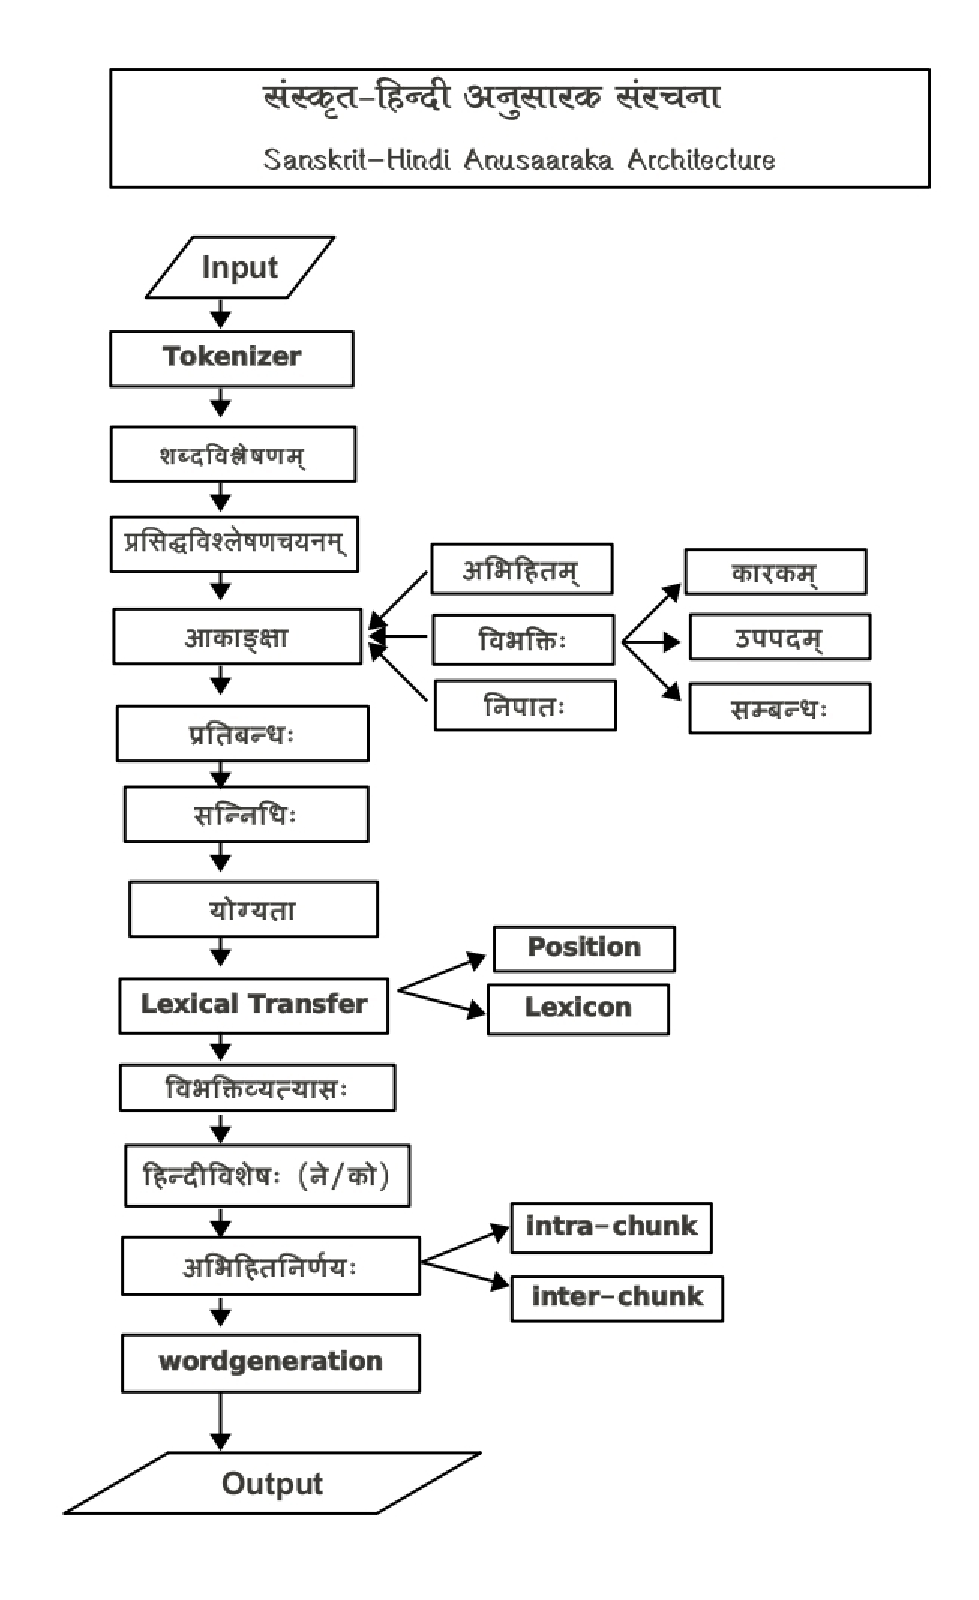
\includegraphics[scale=0.50]{anu_archi.eps}
\end{center}
\end{figure}

\subsection{Module 1: Format Saver and Tokeniser}
This module preserves the formatting information such as tags associated with the words, paragraph markers, display properties such as bold, italic etc.\\

\noindent 
It also adds a sentence tag where the sentence is terminated by any of these punctuation marks viz. [.?!]. \\

\noindent 
Here is a sample input file:\\

\noindent 
Sample Input in WX notation:\\
$<$TITLE$>$ rAma rAma $<$/TITLE$>$\\
$<$p$>$ aham gqham gawvA pATam paTiRyAmi. $<$/p$>$\\
$<$p$>$ rAmaH gqhe nAswi. $<$/p$>$\\

\noindent 
Output:\\
Output contains 4 fields separated by `tabs':\\
$1^{st}$ Field (ID): Identifier with 3 fields separated by `.' indicating paragraph\_number, sentence\_number and word\_number respectively.\\
$2^{nd}$ Field (LTAG): The punctuation marks and the tags to the left of the word.\\
$3^{rd}$ Field (TOKEN): The word.\\
$4^{th}$ Field (RTAG): The punctuation marks and the tags to the right of the word.\\

\noindent 
The output corresponding to the above file is:\\
\begin{verbatim}
1.1.1   <TITLE> rAma
1.1.2           rAma    </TITLE>

2.1.1   <p><s>  aham
2.1.2           gqham
2.1.3           gawvA
2.1.4           pATam
2.1.5           paTiRyAmi       .</s></p>

3.1.1   <p><s>  xaSaraWapuwraH
3.1.2           rAmaH
3.1.3           gqhe
3.1.4           nAswi   .</s></p>

\end{verbatim}
A blank line is a terminator for a sentence.

\subsection{Module 2: Sandhi splitter}

\noindent 
This module is invoked only when the input text type is `sandhied'. 

\noindent 
Sandhi splitter splits the sandhied-words as well as compounds. A compound is split with `-' between the components.
For example, in the previous example, the  word `nAswi' is in sandhied form.
So this is split into two words as `na aswi' as shown below. Similarly the compound word `xaSaraWapuwraH' is split into components as `xaSaraWa-puwraH'.

\begin{verbatim}
1.1.1   <TITLE> rAma
1.1.2           rAma    </TITLE>

2.1.1   <p><s>  aham
2.1.2           gqham
2.1.3           gawvA
2.1.4           pATam
2.1.5           paTiRyAmi       .</s></p>

3.1.1   <p><s>  xaSaraWa-puwraH
3.1.2           rAmaH
3.1.3           gqhe
3.1.4           na
3.1.5           aswi   .</s></p>
\end{verbatim}

\noindent 
At this stage if a sandhied word is split into two or more, then the word numbering gets changed.

\subsection{Module 3: Morph Analyser}

\noindent 
Morph analyser performs 4 tasks:\\
a) Produce inflectional analysis\\
b) Prune the answers\\
c) Use local morph analysis to handle unrecognised words\\
d) Produce derivational analysis of the derived roots\\

\noindent 
Input: \\
Output of the sandhi splitter (or the formatter, if sandhi splitter is not called) is an input to this module. Thus the input is in the form of a table with 4 fields, each field separated by a tab. The output of a sentence is terminated by a blank line.

\noindent 
The four fields are:\\
$1^{st}$ Field (ID): Identifier with 3 fields separated by `.' indicating paragraph\_number, sentence\_number and word\_number respectively.\\
$2^{nd}$ Field (LTAG): The punctuation marks and the tags to the left of the word.\\
$3^{rd}$ Field (TOKEN): The word.\\
$4^{th}$ Field (RTAG): The punctuation marks and the tags to the right of the word.\\

\noindent 
Output:\\
Output consists of 7 fields -- the first four fields are the same as those in the input. Morph analyser adds three more fields corresponding to the inflectional morph analysis (MO\_MW), inflectional morph analysis after pruning (MO\_Apte), and morph analysis after adding the derivational information (MO\_Deri).

\noindent 
The MO\_MW has all possible answers, the pr\={a}tipadikas are from the Monier Williams Dictionary. MO\_Apte prunes out answers corresponding to rare pr\={a}tipadikas (pr\={a}tipadikas not found in Apte's dictionary). MO\_Deri supplies the analysis of words after adding the derivational morph output if the pratipadika is derivational.

\noindent 
These outputs are stored as columns 5, 6 and 7 respectively.

\noindent 
Since the output of later modules depends on the output of the morphological analyser heavily, a provision is made to supply analysis of unrecognised words manually. This anaysis is provided by the user, and then is used by later modules.
This analysis, when available, is copied to the  6th column, and also carried to the 7th column.\\
asmax $<$ vargaH:sarva $><$ lifgam:a $><$ viBakwiH:1 $><$ vacanam:1 $><$ level:1$>$\\
gqha $<$ vargaH:nA $><$ lifgam:napuM $><$ viBakwiH:1 $><$ vacanam:1 $><$ level:1 $>$ / 
gqha $<$ vargaH:nA $><$ lifgam:napuM $><$ viBakwiH:2 $><$ vacanam:1 $><$ level:1 $>$\\
gam1 $<$ vargaH:avy $><$ kqw\_prawyayaH:kwvA $><$ XAwuH:gamLz $><$ gaNaH:BvAxiH $><$ level:1 $>$\\
pATa $<$ vargaH:nA $><$ lifgam:puM $><$ viBakwiH:2 $><$ vacanam:1 $><$ level:1 $>$\\
paT1 $<$ prayogaH:karwari $><$ lakAraH:lqt $><$ puruRaH:u $><$ vacanam:1 $><$ paxI:parasmEpaxI $><$ XAwuH:paTaz $><$ gaNaH:BvAxiH $><$ level:1 $>$\\
 
\noindent 
In case of derivational morphology, the k\d{r}t\_pr\={a}tipadikas and taddhita\_pr\={a}tipadikas are analysed further for k\d{r}t/taddhita analysis.\\

\noindent 
Thus, for example for a word `KAxan' the output is as follows:\\
KAx1 $<$ kqw\_prawyayaH:Sawq $><$ XAwuH:KAxqz $><$ gaNaH:BvAxiH $><$ level:0 $><$ kqw\_pratipadika:KAxaw $><$ vargaH:nA $><$ lifgam:puM $><$ viBakwiH:1 $><$ vacanam:1 $>$ /
KAx1 $<$ kqw\_prawyayaH:Sawq $><$ XAwuH:KAxqz $><$ gaNaH:BvAxiH $><$ level:0 $><$ kqw\_pratipadika:KAxaw $><$ vargaH:nA $><$ lifgam:puM $><$ viBakwiH:8 $><$ vacanam:1 $>$\\

\noindent 
Features corresponding to various parts of speech and the allowed range of values are specified in the morph manual and also available here in appendix (A).\\

\subsection{Module 4: Parser}
Parser takes the input of the morph layer, and produces the correct morph analysis in the context along with the k\={a}raka analysis in fields 8 (Morph\_in\_context) and 9 (k\={a}raka\_analysis) respectively.

\noindent 
Thus the output of the parser for the previous sentences is shown below.
(Only column nos. 3, 8 and 9 are shown)

\begin{verbatim}
aham	asmax<vargaH:sarva><lifgam:a><viBakwiH:1><vacanam:1><level:1>   karwA,5
gqham	gqha<vargaH:nA><lifgam:napuM><viBakwiH:2><vacanam:1><level:1>   karma,3
gawvA	gam1<vargaH:avy><kqw\_prawyayaH:kwvA><XAwuH:gamLz>
	<gaNaH:BvAxiH><level:0>					   pUrvakAlaH,5
pATam	pATa<vargaH:nA><lifgam:puM><viBakwiH:2><vacanam:1><level:1>     karma,5
paTiRyAmi	paT1<prayogaH:karwari><lakAraH:lqt><puruRaH:u>
		<vacanam:1><paxI:parasmEpaxI><XAwuH:paTaz>
		<gaNaH:BvAxiH><level:1> 		       aBihiwa_karwA,1

xaSaraWa-puwraH	xaSaraWa-puwra<vargaH:nA><lifgam:puM><viBakwiH:1>
		<vacanam:1><level:1> viSeRaNam,2
rAmaH           rAma<vargaH:nA><lifgam:puM><viBakwiH:1><vacanam:1>
		<level:1>     karwA,5
gqhe            gqha<vargaH:nA><lifgam:napuM><viBakwiH:7><vacanam:1>
		<level:1>   aXikaraNam,5
na              na<vargaH:avy><level:1> sambanXaH,5
aswi		as2<prayogaH:karwari><lakAraH:lat><puruRaH:pra>
		<vacanam:1><paxI:parasmEpaxI><XAwuH:asaz>
		<gaNaH:axAxiH><level:1>				aBihiwa_karwA,1
\end{verbatim}

\subsection{Module 5: Shallow Parser}
If a parser fails on any input, then shallow parser does minimum parsing of the sentence, and produces pruned morph output to the next layer.

\subsection{Module 6: Word Sense Disambiguation}
This module does the sense disambiguation of root, vibhakti and lak\={a}ra. Sense tags such as `\_1', `\_2' etc. are added to the disambiguated entities. This output is in the same form as of morph. The output is stored in the $10^{th}$ column.

\subsection{Module 7: POS}
This layer in fact is not needed. But is being used just for evaluating the POS tagger. The POS tagger output is stored in the $11^{th}$ column.
At this layer color code is also added. This is needed to display proper color in the interface. Color code information is added to the $12^{th}$ column.

\noindent 
Sample output after this layer is shown below. (Only columns 3, 11 and 12)
\begin{verbatim}
xaSaraWasya	nAma-saM	N6
puwraH	nAma	N1
rAmaH	nAma-saM	N1
nagare	nAma	N7
koSAw	nAma	N5
haswena	nAma	N3
brAhmaNAya	nAma	N4
gAM	nAma	N2
xaxAwi	kriyA	KP
\end{verbatim}

\subsection{Module 8: Chunker}
In this layer some minimum grouping of the words such as `gacCawi sma' etc. is done. The output is stored in the $13^{th}$ column. We show below only the relevant columns viz. $10^{th}$ column in the input and the $13^{th}$ column in the output.

\noindent 
input:
\begin{verbatim}
rAma<vargaH:nA><lifgam:puM><viBakwiH:1><vacanam:1><level:1>
    <rel_nm:karwA><relata_pos:3>
vana<vargaH:nA><lifgam:napuM><viBakwiH:2><vacanam:1><level:1>
    <rel_nm:karma><relata_pos:3>
gam1<prayogaH:karwari><lakAraH:lat><puruRaH:pra><vacanam:1>
    <paxI:parasmEpaxI><XAwuH:gamLz><gaNaH:BvAxiH><level:1>
    <rel_nm:aBihiwa_karwA><relata_pos:1>
sma<vargaH:avy><level:1><rel_nm:sambanXaH><relata_pos:3>
\end{verbatim}

\noindent 
Output:
\begin{verbatim}
rAma<vargaH:nA><lifgam:puM><viBakwiH:1><vacanam:1><level:1>
    <rel_nm:karwA><relata_pos:3>
vana<vargaH:nA><lifgam:napuM><viBakwiH:2><vacanam:1><level:1>
    <rel_nm:karma><relata_pos:3>
gam1<prayogaH:karwari><lakAraH:lat_sma><puruRaH:pra><vacanam:1>
    <paxI:parasmEpaxI><XAwuH:gamLz><gaNaH:BvAxiH><level:1>
    <rel_nm:aBihiwa_karwA><relata_pos:1>
-
\end{verbatim}

\subsection{Module 9: Hindi Lexical Transfer}
In this module, the Sanskrit lexicon is mapped to the corresponding Hindi lexicon. The output now is in the format as required by the Hindi generator. The output is stored in column number 14.
Here are the column numbers 13 and 14 as input and output.

\noindent 
input:
\begin{verbatim}
rAma<vargaH:nA><lifgam:puM><viBakwiH:1><vacanam:1><level:1>
    <rel_nm:karwA><relata_pos:3>
vana<vargaH:nA><lifgam:napuM><viBakwiH:2><vacanam:1><level:1>
    <rel_nm:karma><relata_pos:3>
gam1<prayogaH:karwari><lakAraH:lat_sma><puruRaH:pra><vacanam:1>
    <paxI:parasmEpaxI><XAwuH:gamLz><gaNaH:BvAxiH><level:1>
    <rel_nm:aBihiwa_karwA><relata_pos:1>
\end{verbatim}

\noindent 
output:
\begin{verbatim}
rAma n m s a 0
vana n m s a ko
jA v m s a wA_WA
-
\end{verbatim}

\subsection{Module 10: Hindi Generator}
Hindi generator has two main tasks:

\noindent 
a) Sentence level generation: 
This involves agreement between noun and adjectives, adding `ne', dropping `ko' at unnecessary places, handling kriy\={a}m\={u}la vibhakti and agreement, handling agreement for \d{s}a\d{s}\d{t}{\=\i} vibhaki, kart\={a} and kart\={a}\_sam\={a}n\={a}dhikara\d{n}a, and finally agreement between the noun and the verb.\\

\noindent 
b) Word level generation: At this level, proper form of the word is generated.

\noindent 
Sample input (Only column 14 is shown)
\begin{verbatim}
sIwA n f s a 0
vana n m s a ko
jA v m s a wA_hE

sIwA n f s a 0
rAma n m s a ko
anusaraNa_kara v m s a wA_hE
\end{verbatim}
output after a) (Only column 15 is shown)
\begin{verbatim}
sIwA n f s a 0
vana n m s a ko
jA v f s a wA_hE

sIwA n f s a 0
rAma n m s a kA
anusaraNa_kara v f s a wA_hE

\end{verbatim}
output after b) (Only column 16 is shown)
\begin{verbatim}
sIwA
vana
jAwI_hE

sIwA
rAma_kA
anusaraNa_karawI_hE
\end{verbatim}

\subsection{Module 11: Interface display}
The interface display takes the output in various columns, and produces an xml document that is converted to an html file later.
The output is converted to Roman Diacritic / Devanagari, as per the user's choice. Further the morph o/p and the k\={a}raka relations are transferred to human readable form at this stage.

\section{Evaluation}
The subjective evaluation of the anusaaraka system will be carried out for comprehensibility and the quality, on a scale of 1 to 5. 
Appendix  describes the scale and evaluation metric.

\appendix
\section{File Names: Input, Output and Intermediary}
The input text in the HTML form is stored in /tmp area. The file is named after the process\_id with `in' as a prefix. Corresponding to each input it generates the following files, where PID is the process ID.
\begin{itemize}
\item inPID -- This contains the original text.
\item inPID.wx  -- This contains the text converted to WX notation.
\item inPID.html  -- This contains the anusaaraka layered output.
\item inPID\_trnsltn.html	-- This contains the final Hindi translation.
\item inPID\_frame.html	 -- This is the frame invoking various source files.
\item inPID\_src.html	-- This contains the original text in html format.
\end{itemize}
In addition, there are css and js files which describe the style and contain java script for various effects in the output. These files are copied to the ~user-id/public\_html/scl/SHMT/DEMO. All the intermediate files are stored in tmp\_inPID directory which can later be removed.

\section{Morph output specifications}
The morph analysis is produced as root followed by feature structure.
Feature Structure is an attribute/value pair. Multiple feature structures are separated by '|'.

\subsubsection{Inflectional Morphology}
According to P{\=a}\d{n}ini there are only two basic categories at the level of inflectional morphology. However, for the sake of computational purpose, we also consider avyaya as one of the categories. Later, when we would deal with the Vedic Sanskrit, we may require an additional category, upasarga.\\

\noindent 
The basic categories for morphological analysis of Sanskrit, therefore, are 

\begin{itemize}
\item n{\=a}mapada (noun)
\item kriy{\=a}pada (verb)
\item avyaya (indeclinable)
\item upasarga (pre-position?)
\end{itemize}

\noindent 
\textit {Inflectional morphology}\\
sup:  rt,vargaH,lifgam,viBakwiH,vacanam,level \\
wif:  rt,XAwuH,lakAraH,prayogaH,puruRaH,vacanam,paxI,gaNaH,sanAxiH,level \\
avy:  rt,level \\
upasarga:  rt,level (Note: This category is required only for Vedic Sanskrit literature.)\\

\noindent 
\textit {Derivational morphology}\\
avywaxXiwa: rt,waxXiwa\_prawyayaH,lifgam,level \\
avykqw: rt,kqw\_prawyayaH,XAwuH,gaNaH,level,sanAxiH \\
kqw:  rt,kqw\_prawyayaH,lifgam,viBakwiH,vacanam,XAwuH,gaNaH,kqw\_vb\_rt,level\\
waxXiwa: rt,waxXiwa\_prawyayaH,waxXiwa\_rt,lifgam,viBakwiH,vacanam,level\\

\noindent 
The values of each of these features for Sanskrit is given below.\\
\begin{itemize}
\item vargaH
\begin{itemize}
\item nA (a n{\=a}mapada)
\item sarva (a sarvan{\=a}ma)
\item saMKyeyam (a cardinal number as an adjective)
\item saMKyA (a cardinal number)
\item pUraNam (an ordinal number)
\item avy  (An avyaya)
\end{itemize}
In case of derivational morphology, we indicate finer category information. Following are the subcategories of noun.
\begin{itemize}
\item sa-pU-pa  (sam{\=a}sa p{\=u}rva pada)
\item sa-u-pa-puM (sam{\=a}sa uttarapada in pulli\.{n}ga)
\item sa-u-pa-napuM (sam{\=a}sa uttarapada in napunsakali\.{n}ga)
\item sa-u-pa-swrI (sam{\=a}sa uttarapada in str{\=\i}li\.{n}ga)
\item nA\_mawup (derived taddhita)
\item nA\_wva (derived taddhita)
\item nA\_wamap (derived taddhita)
\item nA\_warap (derived taddhita)
\item nA\_mayat (derived taddhita)
\item nA\_wal (derived taddhita)
\item nA\_kAra (derived compound)
\item nA\_wqc (derived k\d{r}danta)
\item nA\_Sawq (derived k\d{r}danta)
\item nA\_kwavawu (derived k\d{r}danta)
\end{itemize}

\item li\.{n}gam
\begin{itemize}
\item puM
\item swrI
\item napuM
\item a (to indicate any possible lifgam, e.g. in case of sarvan{\=a}ma asmad)
\end{itemize}

\item vacanam
\begin{itemize}
\item 1 (ekavacanam)
\item 2 (dvivacanam)
\item 3 (bahuvacanam)
\end{itemize}

\item puru\d{s}a\d{h}
\begin{itemize}
\item u (uttama)
\item ma (madhyama)
\item pra (prathama)
\end{itemize}

\item vibhakti\d{h}
\begin{itemize}
\item 1 (pratham{\=a})
\item 2 (dvit{\=\i}y{\=a})
\item 3 (t\d{r}tiy{\=a})
\item 4 (caturth{\=\i})
\item 5 (pa\~ncam{\=\i})
\item 6 (\d{s}a\d{s}\d{t}h{\=\i})
\item 7 (saptam{\=\i})
\item 8 (sambodhana)
\end{itemize}

\item lak{\=a}ra
\begin{itemize}
\item lat
\item lit 
\item lut
\item lqt
\item lot
\item laf
\item viXilif
\item ASIrlif
\item luf
\item lqf
\end{itemize}

\item pad{\=\i}
\begin{itemize}
\item AwmanepaxI
\item parasmEpaxI
\end{itemize}

\item prayogaH
\begin{itemize}
\item karwari
\item karmaNi
\item BAve
\end{itemize}

\item gaNa
\begin{itemize}
\item 1  BvAxiH
\item 2  axAxiH
\item 3  juhowyAxiH
\item 4  xivAxiH
\item 5  svAxiH
\item 6  wuxAxiH
\item 7  ruXAxiH
\item 8  wanAxiH
\item 9  kryAxiH
\item 10 curAxiH
\end{itemize}

List of dh\={a}tu\_with\_it will be given in an appendix.\\

\item kqw\_prawyayaH
\begin{itemize}
\item wqc
\item wumun
\item wavyaw
\item yak
\item Sawq
\item SAnac
\item GaF
\item Namul
\item Nvul
\item Nyaw
\item lyut
\item yaw
\item kwvA
\item lyap
\item kwa
\item kwavawu
\item anIyar
\end{itemize}

\item waxXiwa\_prawyayaH
\begin{itemize}
\item wal
\item mawup
\item warap
\item wamap
\item wva
\item vaw
\item wasil
\item karam
\item arWam
\item pUrvaka
\item mayat
\item vAram
\item kqwvasuc
\item xA
\item Sas
\end{itemize}

\subsubsection{Derivational Morphology}
Here are a few examples of the derivational morphology.
\begin{itemize}
\item 
pATayawi	paT1\_Nic $<$ prayogaH:karwari $><$ lakAraH:lat $><$ puruRaH:pra$>$
		$<$ vacanam:1 $><$ paxI:parasmEpaxI $><$ XAwuH:paTaz $>$
		$<$ gaNaH:BvAxiH $><$ level:1 $>$

\item
Agawya   Af\_gam1 $<$ vargaH:avy $><$ kqw\_prawyayaH:lyap $><$ XAwuH:gamLz $>$
	 $<$ gaNaH:BvAxiH $><$ level:1 $>$

\item
XanavawA    Xana $<$ vargaH:nA $><$ waxXiwa\_prawyayaH:mawup $><$ lifgam:puM>
	    $<$ viBakwiH:3 $><$ vacanam:1 $><$ level:3 $>$ /
	    Xana $<$ vargaH:nA $><$ waxXiwa\_prawyayaH:mawup $>$ 
	    $<$ lifgam:napuM $><$ viBakwiH:3 $><$ vacanam:1 $><$ level:3 $>$

\item
gacCawi    gam1 $<$ lifgam:puM $><$ kqw\_prawyayaH:Sawq $><$ XAwuH:gamLz $>$ 
	   $<$ gaNaH:BvAxiH $><$ viBakwiH:7 $><$ vacanam:1 $><$ level:2 $>$ / 
	   gam1 $<$ lifgam:napuM $><$ kqw\_prawyayaH:Sawq $><$ XAwuH:gamLz $>$
	   $<$ gaNaH:BvAxiH $><$ viBakwiH:7 $><$ vacanam:1 $><$ level:2 $>$ / 
	   gam1 $<$ prayogaH:karwari $><$ lakAraH:lat $><$ puruRaH:pra $>$
	   $<$ vacanam:1 $><$ paxI:parasmEpaxI $><$ XAwuH:gamLz $>$ 
	   $<$ gaNaH:BvAxiH $><$ level:1 $>$

\end{itemize}
\end{itemize}
\end{document}
